\documentclass[11pt]{scrartcl}

\usepackage[sexy]{evan}
\usepackage{import}
\usepackage[table]{xcolor}
\usepackage{xfp}
\usepackage{multicol}

\newcommand{\gad}{\textcolor{yellow}{$\bigstar$}}
\newcommand{\bad}{\textcolor{red}{$\bigstar$}}

\definecolor{dcol0}{HTML}{C8E6C9}
\definecolor{dcol1}{HTML}{D4E9B3}
\definecolor{dcol2}{HTML}{E5ED9A}
\definecolor{dcol3}{HTML}{FFF59D}
\definecolor{dcol4}{HTML}{FFE082}
\definecolor{dcol5}{HTML}{FFCC80}
\definecolor{dcol6}{HTML}{FFAB91}
\definecolor{dcol7}{HTML}{F49890}
\definecolor{dcol8}{HTML}{E57373}
\definecolor{dcol9}{HTML}{D32F2F}

\makeatletter
\newcommand{\getcolorname}[1]{dcol#1}
\makeatother

\newcommand{\dif}[1]{%
    \edef\colorindex{\number\fpeval{floor(#1)}}%
    \edef\fulltext{#1}%
    \colorbox{\getcolorname{\colorindex}}{%
        \ifnum\colorindex>8
            \textbf{\textcolor{white}{\,\fulltext\,}}%
        \else
            \textbf{\textcolor{black}{\,\fulltext\,}}%
        \fi
    }%
}
% Variable para dificultad (inicial 0)
\newcommand{\thmdifficulty}{0}

% Comando para asignar dificultad antes del problema
\newcommand{\problemdiff}[1]{\renewcommand{\thmdifficulty}{#1}}

% Estilo del problema que incluye dificultad antes del título
\declaretheoremstyle[
    headfont=\color{blue!40!black}\normalfont\bfseries,
    headformat={%
      \dif{\thmdifficulty}\quad \NAME~\NUMBER\ifx\relax\EMPTY\relax\else\ \NOTE\fi
    },
    postheadspace=1em,
    spaceabove=8pt,
    spacebelow=8pt,
    bodyfont=\normalfont
]{problemstyle}

    \declaretheorem[style=problemstyle,name=Problema,sibling=theorem]{problema}
    \declaretheorem[style=problemstyle,name=Problema,numbered=no]{problema*}

\definecolor{yellow4}{RGB}{255, 206, 0}

\title {Principio Extremo}
\subtitle {Entrenamientos Nacionales Platas y EGMOs}

\author{Emmanuel Buenrostro}
\date{9 de Enero de 2026}

\begin{document}
\maketitle

\section{¿Qué es?}
Este tecnica consiste en tomar objetos con propiedades \textbf{extremas} para resolver problemas, esto sirve particularmente 
para problemas que tengan una cantidad finita de objetos. \\


Pero ¿A qué nos referimos con propiedades extremas?, te tomas alguna propiedad medible y un conjunto de objetos en los cuales puedes medir esa propiedad, entonces 
lo que haces es trabajar con los objetos que tengan el máximo o el minimo de esa propiedad y te pueden dar cosas útiles enfocarte en esos objetos particularmente.  \\

Ejemplos de propiedades: 

\begin{itemize}
    \item Longitud minima/maxima entre dos puntos
    \item Área minima/maxima de algunos poligonos.
    \item Menor/Mayor divisor primo
    \item Mayor/Menor grado de un vertice en un grafo.
    \item Mayor/menor cantidad de casillas de cierto color en un tablero.
    \item \ldots.
\end{itemize}


Algo que hay que tener cuidado es que en verdad existan esos extremos, por ejemplo no existe un maximo número entero, un mínimo número real positivo, etc.  \\
Casos en los que existen esos extremos son:  los conjuntos finitos (ambos), en enteros positivos existe un minimo.

\section{Ejemplos}

\begin{example} [Tomar un mínimo / máximo]
    En un plano, cada punto con coordenadas enteras es nombrado con un entero positivo, de manera que el número en cada punto es el promedio de sus 4 vecinos. Demuestra que todas los puntos tienen el mismo número.
\end{example}

\begin{soln}
Como son enteros positivos, existe una etiqueta positiva $m$, y digamos que las etiquetas a su alrededor son $a,b,c,d$, como $m$ es minima entonces $a,b,c,d \geq m$ y sabemos que 
\[m=\frac{a+b+c+d}{4} \geq \frac{4m}{4}=m\]
Entonces $a=b=c=d=m$ y se va expandiendo por todo el plano para ver que todas son iguales.
\end{soln}
\begin{remark*}
Tomar la etiqueta minima es posible debido a que son enteros positivos, pero si fueran enteros si existiria un acomodo que no lleva a que todas son iguales nombrando a $(x,y)$ como $x+y$.  
\end{remark*}

\begin{example} [OMM 2024/5]
    Sean $A$ y $B$ conjuntos infinitos de números reales positivos tales que:
    \begin{itemize}
        \item Para cualquier par de elementos $u \geq v$ de $A$, se cumple que $u+v$ es elemento de $B$.
        \item Para cualquier par de elementos $s > t$ de $B$, se cumple que $s-t$ es elemento de $A$.
    \end{itemize}
    Prueba que $A=B$ o existe un número real $r$ tal que $B=\{2r,3r,4r,\ldots\}$.
\end{example}
\begin{soln}
¿Podemos tomar el elemento minimo de $A$ o $B$?\\
\textbf{NO}, ya que son conjuntos \textbf{infinitos} de reales positivos, un ejemplo de un conjunto infinito de reales positivos es $(0,1)$, el cual no tiene minimo ni maximo, ya que no importa que tanto te acerques a $0$ o a $1$, siempre va a haber un real mas pequeño/grande en el conjunto pero que nunca 
llegara a $0$ o $1$. Por esta razón no existen elementos minimos o máximos, tomarse un elemento minimo / ordenar los elementos fue un error que mucha gente cometio en ese nacional y causo muchos fakesolves.  \\
(Si les interesa la solución si usa el caso de cuando tomas el elemento minimo, y el caso de cuando no tiene pero no la vamos a ver ahorita.)
\end{soln}

\begin{example} [Demostrar infinidad]
    Sea $\Omega$ un conjunto de puntos en el plano, tal que cualquier punto en $\Omega$ es el punto medio del segmento formado por dos puntos de $\Omega$. Demuestra que $\Omega$ tiene infinitos puntos
\end{example}
\begin{soln}
    Si un conjunto es finito, sabemos que existe un máximo y un mínimo, entonces demostrar que no existe alguno de estos 
    es suficiente para probar que un conjunto es infinito. \\
    Entonces asumamos que $AB$ tiene la distancia máxima entre los segmentos formados por dos puntos en $\Omega$, con $A,B \in \Omega$. Sabemos que $B$ es punto medio de $CD$ con $C,D \in \Omega$.  Alguno de los ángulos $\angle ABC, \angle ABD$ es al menos $90^{\dg}$. Entonces al menos una de $AC,AD$ es mayor a $AB$, contradicción, por lo tanto el conjunto es infinito.  \\

\end{soln}


\begin{example}
    [Dar un acomodo]
    Hay $2n$ puntos en el plano, de forma que no hay 3 colineales. $n$ son coloreados de azul y $n$ de rojo. Demuestra que puedes unir los $n$ puntos rojos a los $n$ puntos azules con $n$ segmentos (cada segmento une un punto rojo con uno azul), de forma que no hay dos segmentos que se intersecten. 
\end{example}

\begin{soln}
    Esta vez vamos a tomarnos un acomodo que minimice algo, en este caso vamos a minimizar la suma de los $n$ segmentos utilizados. \\
    Veamos que este acomodo funciona, ya que si dos segmentos $AB,CD$ se intersectan en $P$. Podemos ver que por desigualdad del triangulo: 

    \[AB+CD=AP+PB+CP+PD=(AP+PD)+(CP+PB) > AD+CB\]
    \begin{center}
        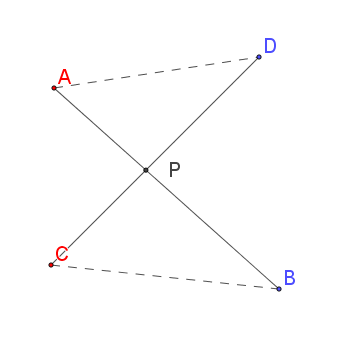
\includegraphics[scale=0.5]{IMG1.png}
    \end{center}
    Podrias tomar ese acomodo y haria que la suma sea menor, contradiciendo la minimicidad del acomodo, entonces ese acomodo si cumple las condiciones.

\end{soln}

En estos ultimos problemas, tenemos un conjunto finito de cosas, pero no hacemos principio extremo sobre ese conjunto, si no sobre "combinaciones" de esos conjuntos, ya que estas combinaciones tambien son \textbf{finitas}.


\begin{remark*}
    La mayoria de los argumentos de descenso infinito tambien pueden ser expresados como argumentos de principio extremo.
\end{remark*}

\newpage
\section{Problemas}
\epigraph{El tiempo solo sana lo que ya no importa}{"Como pasa el tiempo" - Cuarteto de nos}

\section{Nivel I}
\problemdiff{1}
\begin{problem}
    Determina cuales de estos conjuntos tienen minimo, y cuales tienen maximo. 
    \begin{multicols}{2}
    \begin{itemize}
        \item Enteros 
        \item Enteros positivos 
        \item Enteros no negativos 
        \item Enteros negativos 
        \item Racionales  
        \item Racionales positivos 
        \item Reales en $[0,1]$
        \item Reales en $(0,1)$
        \item Reales positivos. 
    \end{itemize}
    \end{multicols}
\end{problem}
\problemdiff{2}
\begin{problem}
    Hay $n$ estudiantes en un salon de tal forma que la distancia entre cada pareja de estudiantes es distinta. Cada estudiante tiene una pelota, y cuando el profesor suena un silbato, cada estudiante lanza su pelota a el estudiante mas cercano a el. Demuestra que hay una pareja de estudiantes que lanzan las pelotas mutualmente.
\end{problem}

\problemdiff{2}
\begin{problem} 
    Sea $x_1,x_2,\ldots,x_n$ una sucesión de enteros positivos tales que no son todos iguales y
    \[\frac{x_{i-1}+x_{i+1}}{x_i}\] es entero para toda $1 \leq i \leq n$ donde $x_0=x_n$ y $x_{n+1}=x_1$.  Demuestra que existe un entero positivo $1 \leq k \leq n$ tal que $x_k=x_{k-1}+x_{k+1}$. 
\end{problem}

\problemdiff{2}
\begin{problem}
    En un entrenamiento de matemáticas hay 6 estudiantes, quienes después de un arduo día de trabajo se sientan formando un circulo. Su astucia matematica les hace darse cuenta 
    de que la edad de cualquiera de ellos es el promedio de las edades de los dos vecinos de esa persona. Demuestra que todos tienen la misma edad.
\end{problem}



\problemdiff{3}
\begin{problem} [\gad]
    Se tienen $n$ puntos en el plano. Cualquiera tres de ellos fomran un triangulo con area menor a $1$. Muestra que todos los puntos estan en un traingulo con un area menor o igual a $4$.
\end{problem}

\problemdiff{3}
\begin{problem}
    En un torneo, todos los equipos jugaron contra todos los demás, en ningun juego hubo empates. Prueba que existe un equipo $A$, tal que cualquier otro equipo le gano o bien le gano a un equipo que le gano a $A$.
\end{problem}


\problemdiff{3}
\begin{problem}
    Hay $n$ estudiantes en un salon, con $n$ impar, de tal forma que la distancia entre cada pareja de estudiantes es distinta. Cada estudiante tiene una pelota, y cuando el profesor suena un silbato, cada estudiante lanza su pelota a el estudiante mas cercano a el. Demuestra que hay un estudiante que no le lanzan ninguna pelota.
\end{problem}

\problemdiff{3}
\begin{problem}
    Sean $a_1,\ldots, a_n$ una sucesión de números reales positivos tal que $a_1=1$ y $a_{n+1}^2+a_{n+1}=a_n$ para todo $n \geq 1$. Muestra que $a_n\geq \frac 1n$ para todo $n$.
\end{problem}

\section{Nivel II}

\problemdiff{4}
\begin{problem}
    Tienes una cantidad finita de puntos rojos y azules en el plano, de manera que cada segmento que une dos putnos del mismo color contiene un punto del otro color. Prueba que todos los puntos son colineales.
\end{problem}

\problemdiff{4}
\begin{problem}
    Para $n>1$, los enteros del $1$ al $n^2$ son colocados en celdas de un tablero de $n\times n$. Prueba que existe un par de celdas adjacentes (vertical, horizontal o diagonalmente) las cuales sus valores difieren por al menos $n+1$.
\end{problem}

\problemdiff{4}
\begin{problem}
    Demuestra que no hay una cuarteta de enteros positivos $(x,y,z,u)$ tales que \[x^2+y^2=3(z^2+u^2)\]
\end{problem}



\problemdiff{4}
\begin{problem}
    Cada calle en Colima es de una dirección. Cada par de ciudades estan conectadas por exactamente una calle. Prueba que existe una ciudad a la que se puede llegar desde cada otra ciudad, ya sea directamente o pasando por a lo más otra ciudad.
\end{problem}

\section{Nivel III}
\problemdiff{5}
\begin{problem}  [EGMO 2021/1]
    
    El número $2021$ es fantabuloso. Si para algún entero positivo $m$, alguno de los elementos del conjunto $\{m, 2m + 1, 3m\}$ es fantabuloso, entonces todos los elementos de dicho conjunto
son fantabulosos. ¿Esto implica que el número $2021^{2021}$ es fantabuloso?
\end{problem}


\problemdiff{5}%??
\begin{problem}
    En una fiesta con $n$ personas, se sabe que entre cualesquiera $4$ personas, hay o bien $3$
personas que se conocen entre sí o bien $3$ personas, tales que ningún par entre ellas se conoce.
Muestra que las $n$ personas se pueden separar en dos salones, de tal forma que en uno todos
se conocen y en el otro nadie conoce a nadie.
\end{problem}

\problemdiff{5}
\begin{problem}
    Sea $a_0 < a_1 <\ldots$  una sucesión infinita de enteros positivos. Muestra que existe un único entero $n \leq 1$ tal que 
    \[a_n < \frac{a_0+a_1+\ldots+a_n}{n} < a_{n+1}\]
\end{problem}

\problemdiff{5}
\begin{problem}
    En todo $n$-agono convexo existen tres vertices consecutivos $ABC$, tal que el circuncirculo de $ABC$ cubre todo el $n$-agono.
\end{problem}

\problemdiff{5}
\begin{problem} %[Balkan 2010/3]
    Una franja de ancho $w$ es el conjunto de todos los puntos que están sobre, o entre, dos rectas paralelas separadas por una distancia $w$. Sea $S$ un conjunto de $n$ puntos ($n \ge 3$) en el plano tal que cualesquiera tres puntos distintos de $S$ pueden ser cubiertos por una franja de ancho $1$.

Demuestra que $S$ puede ser cubierto por una franja de ancho $2$.
\end{problem}

\subsection{Nivel IV}

\begin{problem}
Las sucesiones $a_1,\ldots, a_n$ y $b_1,b_2, \ldots, b_n$ son permutaciones de $1, \frac 12, \frac 13, \ldots, \frac 1n$, además $a_1+b_1 \geq a_2+b_2\geq \ldots \geq a_n+b_n$. Prueba que $a_m+b_m \leq \frac 4m$ para todo $1 \leq m \leq n$.
\end{problem}

\begin{problem}
Hay $n$ estudiantes en cada una de tres escuelas. Cada estudiante conoce a $n+1$ estudiantes de las otras dos escuelas. Prueba que puedes escoger un estudiante de cada escuela, de forma que los 3 se conocen entre si.
\end{problem}

\problemdiff{6}
\begin{problem} %[USA TSTST 2016/5]
    En el plano coordenado hay un número finito de muros, que son segmentos de recta disjuntos entre sí, ninguno de los cuales es paralelo a alguno de los ejes. Un bulldozer comienza en un punto arbitrario y se mueve en la dirección $+x$. Cada vez que golpea un muro, gira en un ángulo recto con respecto a su trayectoria, alejándose del muro, y continúa moviéndose. (Por lo tanto, el bulldozer siempre se mueve paralelo a los ejes).

Demuestra que es imposible que el bulldozer golpee ambos lados de cada muro.
\end{problem}



\end{document}